% -----------------------------------
% -----------------------------------
% abnTeX2: Normas ABNT NBR 14724:2011 + sugestões FGV/EMAp. 

% Autor: Lauro César Araujo
% Adaptações EMAp: Lucas Machado Moschen 
% Copyright 2012-2018 by abnTeX2 group at http://www.abntex.net.br/ 

%% This work may be distributed and/or modified under the
%% conditions of the LaTeX Project Public License, either version 1.3
%% of this license or (at your option) any later version.
%% The latest version of this license is in
%%   http://www.latex-project.org/lppl.txt
%% and version 1.3 or later is part of all distributions of LaTeX
%% version 2005/12/01 or later.
% ----------------------------------
% ----------------------------------
\documentclass[
	% -- opções da classe memoir --
	12pt,				% tamanho da fonte
	%openright,			% capítulos começam em página ímpar (insere página vazia caso preciso)
	oneside,			% para impressão em recto e verso. Oposto a oneside
	a4paper,			% tamanho do papel. 
	% -- opções da classe abntex2 --
	%chapter=TITLE,		% títulos de capítulos convertidos em letras maiúsculas
	%section=TITLE,		% títulos de seções convertidos em letras maiúsculas
	%subsection=TITLE,	% títulos de subseções convertidos em letras maiúsculas
	%subsubsection=TITLE,% títulos de subsubseções convertidos em letras maiúsculas
	% -- opções do pacote babel --
	english,			% idioma para inglês
	%brazil				% idioma para português
	]{abntex2}

%------------------------------------------------
%-------------- Pacotes necessários -------------
%------------------------------------------------

% Escrita 
\usepackage[T1]{fontenc}
\usepackage[utf8]{inputenc}
\usepackage{lmodern}
\usepackage{microtype} % para melhorias de justificação
\usepackage{indentfirst}
\usepackage{csquotes}
% \newtheorem{theorem}{Theorem}[section]

\renewcommand{\ABNTEXchapterfont}{\fontfamily{ptm}\fontseries{b}\selectfont}

% Gráficos 
\usepackage{color}
\usepackage{caption}
\usepackage{subcaption}
\usepackage{multirow}
\usepackage{graphicx}
\usepackage{pdfpages}
\usepackage{cancel}
\usepackage{quiver}

% \usepackage{pgfplots}
\graphicspath{{../../images/}}

% Matemáticos 
\usepackage{bbm}
\usepackage{amsthm, amssymb, amsmath, mathtools}

% Outros 
\usepackage{lipsum}
%\usepackage[textsize=tiny, textwidth=15mm]{todonotes}
\usepackage{multirow}
\usepackage{listings}
\usepackage{lstbayes}
% \usepackage[shortlabels]{enumitem}

% Citações 
%\usepackage[brazilian,hyperpageref]{backref}
%\usepackage[alf]{abntex2cite}	% Citações padrão ABNT
\usepackage[style=abnt]{biblatex}
% \usepackage{natbib}
\addbibresource{biblio.bib}  

% \renewcommand{\backrefpagesname}{Citado na(s) página(s):~}
% % Texto padrão antes do número das páginas
% \renewcommand{\backref}{}
% % Define os textos da citação
% \renewcommand*{\backrefalt}[4]{
% 	\ifcase #1 %
% 		Nenhuma citação no texto.%
% 	\or
% 		Citado na página #2.%
% 	\else
% 		Citado #1 vezes nas páginas #2.%
% 	\fi}%
% ---

%----------------------------------------
%------- Capa e Folha de Rosto ----------
%----------------------------------------

\newcommand\subtitulo[1]{\def\@subtitulo{#1}}
\newcommand{\imprimirsubtitulo}{\@subtitulo}

\renewcommand{\imprimircapa}{%
	\begin{capa}%
	\center
		\ABNTEXchapterfont\Large \MakeUppercase{\imprimirinstituicao}
		\\\vspace*{4cm}
		{\ABNTEXchapterfont\large \MakeUppercase{\imprimirautor}}
		\vfill
		\begin{center}
		\ABNTEXchapterfont\large\MakeUppercase{\imprimirtitulo}\normalfont\MakeUppercase{:
		\imprimirsubtitulo}
		\end{center}
		\vfill
		\normalfont\large\imprimirlocal
		\\\normalfont\large\imprimirdata
		\vspace*{1cm}
	\end{capa}
}

\makeatletter
\renewcommand{\folhaderostocontent}{
  \begin{center}

    %\vspace*{1cm}
    {\ABNTEXchapterfont\large\MakeUppercase{\imprimirautor}}
	
    \vspace*{\fill}\vspace*{\fill}
    \begin{center}
      \ABNTEXchapterfont\bfseries\large\MakeUppercase{\imprimirtitulo}\normalfont\MakeUppercase{:
      \imprimirsubtitulo}
    \end{center}
    \vspace*{\fill}
	
    \abntex@ifnotempty{\imprimirpreambulo}{%
      \hspace{7.5cm}
      \begin{minipage}{.5\textwidth}
      	\SingleSpacing
         \imprimirpreambulo
         \\\\
         Advisor: \imprimirorientador
       \end{minipage}%
       \vspace*{\fill}
    }%

    % {\large\imprimirorientadorRotulo~\imprimirorientador\par}
    % \abntex@ifnotempty{\imprimircoorientador}{%
    %    {\large\imprimircoorientadorRotulo~\imprimircoorientador}%
    % }%
    \vspace*{\fill}

    {\large\imprimirlocal}
    \par
    {\large\imprimirdata}
    \vspace*{1cm}

  \end{center}
}
\makeatother


\titulo{A survey on fully homomorphic encryption with statistical applications}
\autor{Rener de Souza Oliveira}
\local{Rio de Janeiro}
\data{2022}
\instituicao{%
  Fundação Getulio Vargas \\
  \par
  School of Applied Mathematics
}
\tipotrabalho{Bachelor Dissertation (Undergraduation)}

\preambulo{Bachelor dissertation presented to the School of Applied
Mathematics (FGV/EMAp) to obtain the Bachelor's degree in Applied Mathematics.
\\ \\ Areas of Study: Cryptography, Machine Learning}

\orientador{Rodrigo dos Santos Targino}

% Se o seu texto tem subtítulo. 
% Se não tiver, altere o arquivo capa_folha_rosto_tex
% \subtitulo{Training models over encrypted data}

%---------------------------------------------
%-------------------- PDF --------------------
%---------------------------------------------

% alterando o aspecto da cor azul
\definecolor{blue}{RGB}{41,5,195}

% informações do PDF
\makeatletter
\hypersetup{
     	%pagebackref=true,
		pdftitle={\@title}, 
		pdfauthor={\@author},
    	pdfsubject={\imprimirpreambulo},
	    pdfcreator={LaTeX with abnTeX2},
		pdfkeywords={abnt}{latex}{abntex}{abntex2}{trabalho acadêmico}, 
		colorlinks=true,       		% false: boxed links; true: colored links
    	linkcolor=blue,          	% color of internal links
    	citecolor=blue,        		% color of links to bibliography
    	filecolor=magenta,      		% color of file links
		urlcolor=blue,
		bookmarksdepth=4
}
\makeatother

% Posiciona figuras e tabelas no topo da página quando adicionadas sozinhas
% em um página em branco. Ver https://github.com/abntex/abntex2/issues/170
\makeatletter
\setlength{\@fptop}{5pt} % Set distance from top of page to first float
\makeatother

%---------------------------------------
%--------- Mais configurações-----------
%---------------------------------------

% Possibilita criação de Quadros e Lista de quadros.
% Ver https://github.com/abntex/abntex2/issues/176
\newcommand{\quadroname}{Quadro}
\newcommand{\listofquadrosname}{Lista de quadros}

\newfloat[chapter]{quadro}{loq}{\quadroname}
\newlistof{listofquadros}{loq}{\listofquadrosname}
\newlistentry{quadro}{loq}{0}

% configurações para atender às regras da ABNT
\setfloatadjustment{quadro}{\centering}
\counterwithout{quadro}{chapter}
\renewcommand{\cftquadroname}{\quadroname\space} 
\renewcommand*{\cftquadroaftersnum}{\hfill--\hfill}

\setfloatlocations{quadro}{hbtp} % Ver https://github.com/abntex/abntex2/issues/176

%-----------------------------------------------------
%--------------------- Margens -----------------------
%-----------------------------------------------------

\setlrmarginsandblock{3cm}{2cm}{*} % The correct is 3/2
\setulmarginsandblock{3cm}{2cm}{*}
\checkandfixthelayout

%-----------------------------------------------------
%------ Espaçamentos entre linhas e parágrafos -------
%-----------------------------------------------------

% O tamanho do parágrafo é dado por:
\setlength{\parindent}{1.3cm}

% Controle do espaçamento entre um parágrafo e outro:
\setlength{\parskip}{0.2cm}  % tente também \onelineskip

% compila o índice
\makeindex

%------------------------------------------------------
%----------- Personal Definitions ---------------------
%------------------------------------------------------

\newcommand{\Cypher}{\mathcal C }
\newcommand{\Plain}{\mathcal P }
\newcommand{\Z}{\mathbb{Z}}
\newcommand{\R}{\mathbb{R}}
\newcommand{\x}{\boldsymbol{x}}
\newcommand{\N}{\mathbb{N}}
\newcommand{\poly}{\operatorname{poly}}
\newcommand{\bda}{\boldsymbol{a}}
\newcommand{\bds}{\boldsymbol{s}}
\newcommand{\pk}{\operatorname{pk}}
\newcommand{\sk}{\operatorname{sk}}
\newcommand{\enc}{\operatorname{Enc}}
\newcommand{\dec}{\operatorname{Dec}}
% \newcommand{\gcd}{\operatorname{gcd}}
% \newcommand{\betadist}{\operatorname{Beta}}
% \newcommand{\bern}{\operatorname{Bernoulli}}
% \newcommand{\tril}{\operatorname{tril}}

% \newcommand{\ev}{\mathbb{E}}
% \newcommand{\var}{\operatorname{Var}}
% \newcommand{\cor}{\operatorname{Cor}}
% \newcommand{\cov}{\operatorname{Cov}}

% \newcommand{\ind}{\mathbbm{1}}
% \newcommand{\logit}{\operatorname{logit}}

\newtheorem{theorem}{Theorem}[section]
\newtheorem{proposition}{Proposition}[section]
\newtheorem{corollary}{Corollary}[section]
\theoremstyle{definition}
\newtheorem{definition}{Definition}[section]

\theoremstyle{remark}
\newtheorem{remark}{Remark}[section]
\newtheorem{assumption}{Assumption}

\newcommand{\improve}[1]{\textcolor{red}{#1}}

\renewcommand{\quadroname}{Chart}

%-------------------------------------------------
%----------------- Document ----------------------
%-------------------------------------------------

\begin{document}

\newcounter{num}
% if num != 1, do not print the pre textual 
\setcounter{num}{1}

\selectlanguage{english}
\frenchspacing 

%----------------------------------------------
%--------------- Pré-textuais -----------------
%----------------------------------------------
%\pretextual

\imprimircapa

\ifnum\value{num}=1
{\imprimirfolhaderosto*

\begin{fichacatalografica}
	\sffamily
	\vspace*{\fill}					% Posição vertical
	\begin{center}					
	\fbox{\begin{minipage}[c][8cm]{13.5cm}		% Largura
	\small
	Ficha catalográfica elaborada pela BMHS/FGV \\

	%\imprimirautor
	Oliveira, Rener de Souza % Paginas com as citações na bibl
	
	\hspace{0.5cm} \imprimirtitulo / \imprimirautor. -- \imprimirdata.
	
	\hspace{0.5cm} \thelastpage f.\\
		
	\hspace{0.5cm}
	\parbox[t]{\textwidth}{\imprimirtipotrabalho~--~School of Applied
	Mathematics.}\\
	
	\hspace{0.5cm} Advisor: \imprimirorientador .

	\hspace{0.5cm} Includes bibliography. \\
	
	\hspace{0.5cm}
		1. Private Machine Learning.
		2. Fully Homomorphic Encryption.
% 		2. Sensitivity and specificity.
		I. Targino, Rodrigo dos Santos.
		II. School of Applied Mathematics.
		III. \imprimirtitulo 			
	\end{minipage}}
	\end{center}
\end{fichacatalografica}

% Uncomment if you have the pdf 
% \begin{fichacatalografica}
%     \includepdf{fig_ficha_catalografica.pdf}
% \end{fichacatalografica}

%\begin{errata}

\begin{table}[htb]
    \center
    \footnotesize
    \begin{tabular}{|p{1.4cm}|p{1cm}|p{3cm}|p{3cm}|}
    \hline
    \textbf{Folha} & \textbf{Linha} & \textbf{Onde se lê} &
    \textbf{Leia-se}\\
    \hline
    17 & 8 & Matemtica & Matemática \\
    \hline
    \end{tabular}
\end{table}

\end{errata}

% % \begin{folhadeaprovacao}

%     \begin{center}
%       {\ABNTEXchapterfont\large\MakeUppercase{\imprimirautor}}
  
%       \vspace*{\fill}\vspace*{\fill}
%       \begin{center}
%         \ABNTEXchapterfont\bfseries\large\MakeUppercase{\imprimirtitulo}
%       \end{center}
%       \vspace*{\fill}
      
%       \hfill
%       \begin{minipage}{.7\textwidth}
%           \imprimirpreambulo \\ \\
%           Approved on December ----, 2021 \\
%           By the organizing committee
%       \end{minipage}%
%       \vspace*{\fill}
%      \end{center}
  
%      \assinatura{\imprimirorientador \\ School of Applied Mathematics} 
%      \assinatura{Cláudio José Struchiner \\ School of Applied Mathematics}
%      \assinatura{Leonardo Soares Bastos \\ Scientific Computing Program, Oswaldo Cruz Foundation}
%      %\assinatura{\textbf{Professor} \\ Convidado 3}
%      %\assinatura{\textbf{Professor} \\ Convidado 4}
% \end{folhadeaprovacao}

\begin{folhadeaprovacao}
  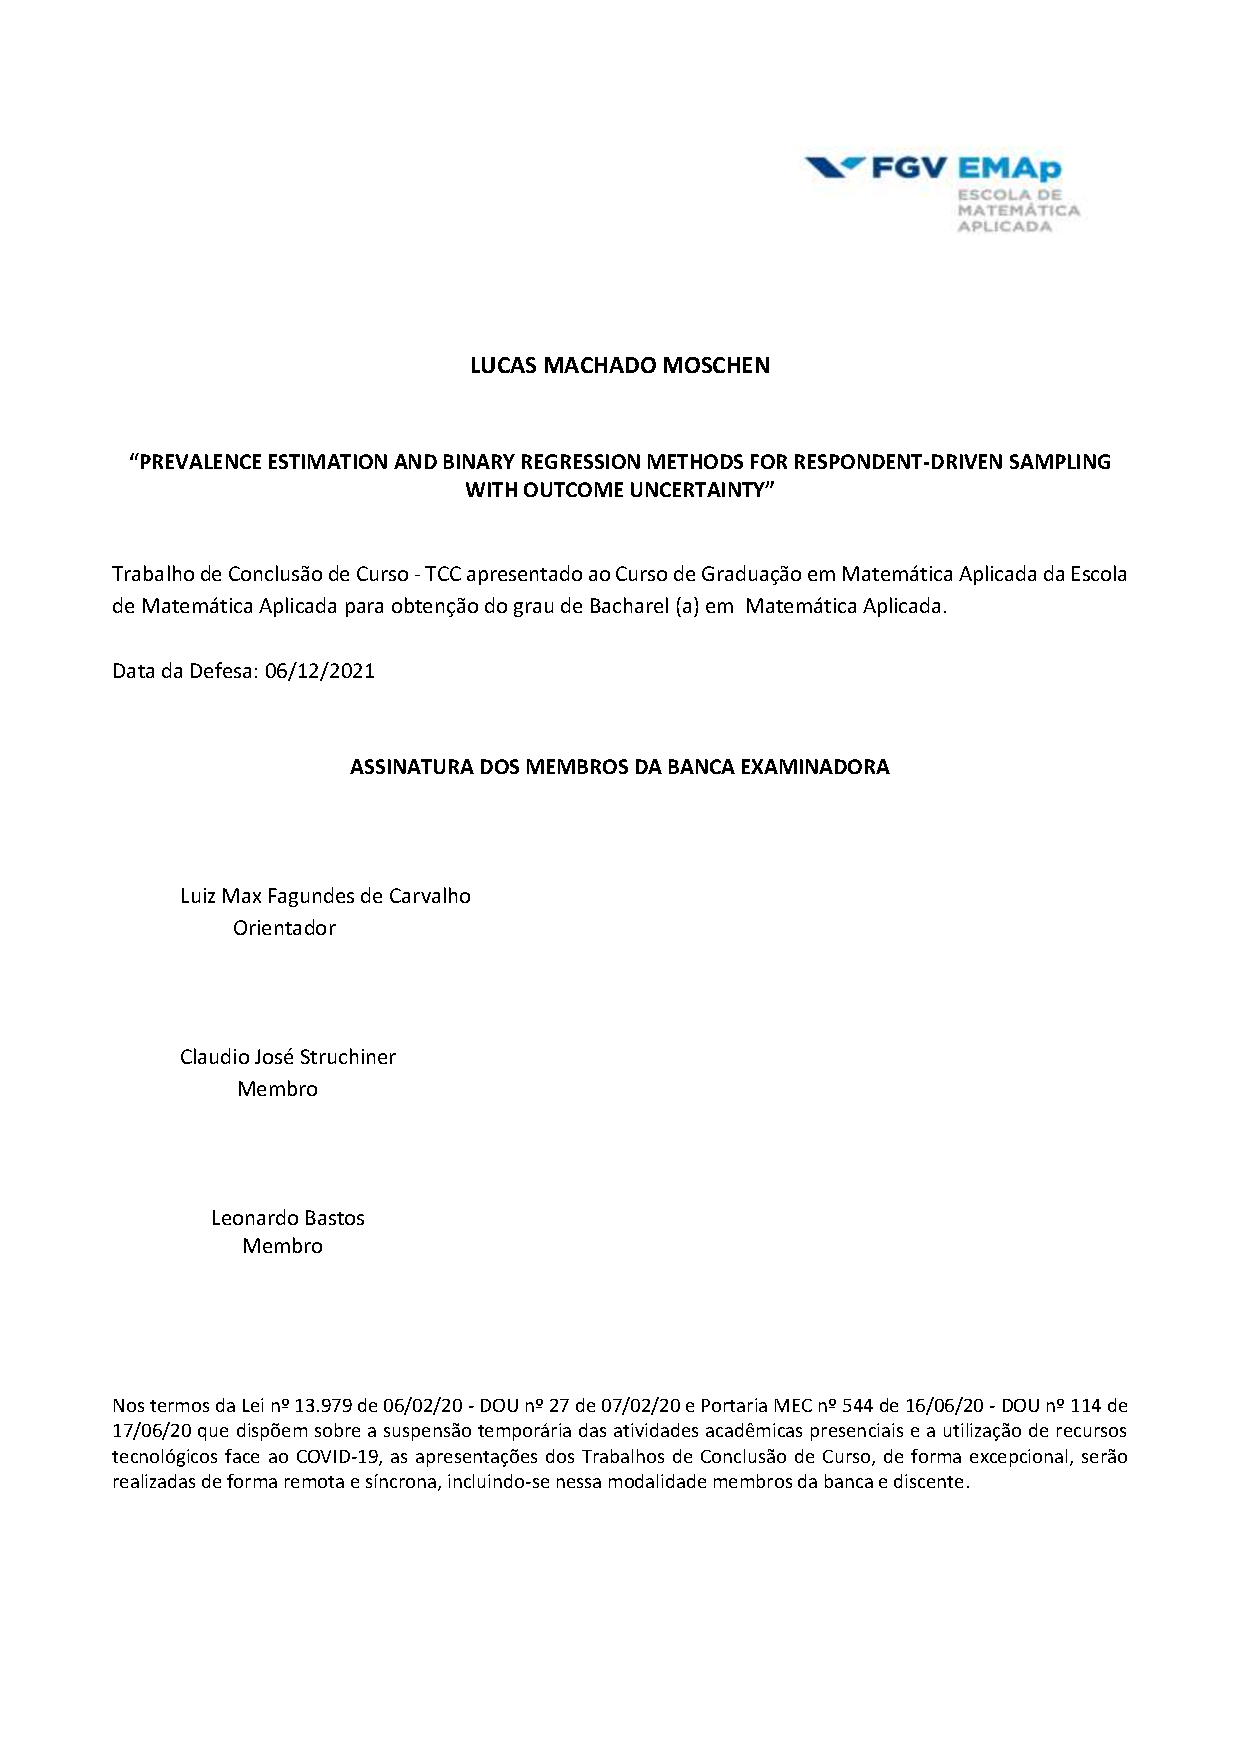
\includepdf{files/folha_aprovacao_nosign.pdf}
\end{folhadeaprovacao}

\newpage

\begin{dedicatoria}
    \vspace*{\fill}
    %\noindent
    \hfill
    \begin{minipage}{.6\textwidth}
        I dedicate this dissertation to you!
    \end{minipage}
\end{dedicatoria}
 
\begin{agradecimentos}
	Thanks, guys!
\end{agradecimentos}

\begin{epigrafe}
\vspace*{\fill}

\begin{flushright}
    \hspace{7.5cm}
    \textit{
        ``One of the pervasive risks that we face in the \\ information age is
        that even if the amount of \\ knowledge in the world is increasing,
        the gap \\ between what we know and what we think \\ we know may be
        widening.''} \\
        \textit{Nate Silver}
\end{flushright}
\end{epigrafe}


\setlength{\absparsep}{18pt} 

\begin{resumo}[Abstract]
 \begin{otherlanguage*}{english}
 The amount of data generated by individuals and enterprises is growing exponentially over the last decades, which empowers the use of machine learning methods since, for statistical purposes, the more data a model can have access to, the more accurately it will predict or represent reality. The problem emerges when the model must deal with sensitive data such as medical records, financial history, or genomic data, in which additional care must be taken in order to protect the privacy of data owners. Encrypting sensitive data might appear a good solution at first sight, but it can considerably limit the ability to do statistical analysis. This work is a survey on \textit{Fully Homomorphic Encryption (FHE)}, a special kind of cryptography scheme that still permits some machine learning methods to run over encrypted data, while it has strong mathematical guarantees of privacy protection.  
 \end{otherlanguage*}

 Keywords: Machine Learning, Cryptography, Fully Homomorphic Encryption, Logistic Regression.
\end{resumo}

\begin{resumo}[Resumo]
    A quantidade de dados gerados por pessoas e empresas está crescendo exponencialmente nas últimas décadas, o que potencializa o uso de métodos de aprendizado de máquina, pois, para fins estatísticos, quanto mais dados um modelo tiver acesso, mais preciso ele será na previsão ou representação da realidade. O problema surge quando o modelo precisa lidar com dados sensíveis, como registros médicos, histórico financeiro ou dados genômicos, nos cuidado adicional deve ser tomado para proteger a privacidade dos proprietários dos dados. Criptografar tais dados, pode parecer uma boa solução à primeira vista, mas pode limitar consideravelmente a capacidade de fazer análises estatísticas. Este trabalho é uma pesquisa sobre \textit{Criptografia Completamente Homomórgica} um tipo especial de esquema de criptografia que permite a execução de alguns modelos de aprendizado sobre dados criptografados, enquanto, ao mesmo tempo, mantém fortes garantias matemáticas de proteção de privacidade.
    
    Palavras-chave: Aprendizado de Máquinas, Criptografia, Criptografia Totalmente Homomórfica, Regressão Logística.
\end{resumo}


\pdfbookmark[0]{\listfigurename}{lof}
\listoffigures*
\cleardoublepage

% \pdfbookmark[0]{\listofquadrosname}{loq}
% \listofquadros*
% \cleardoublepage

\pdfbookmark[0]{\listtablename}{lot}
\listoftables*
\cleardoublepage

\begin{siglas}
    \item[FHE] Fully Homomorphic Encryption
    \item[LHS] Left-hand side
    \item[RHS] Right-hand side  
  \end{siglas}
  
  \begin{simbolos}
    \item[$\in$] Belongs to 
    \item[$\overline{z}$] Complex conjugate of $z$. $\overline{z}=a-bi$ for $z=a+bi$.
  \end{simbolos}


}\fi

\pdfbookmark[0]{\contentsname}{toc}
\tableofcontents*
\cleardoublepage

% ----------------------------------------------------------
% ELEMENTOS TEXTUAIS
% ----------------------------------------------------------
\textual

\chapter{Introduction}

Remember to cite every person \cite{fhe_integers}.




% ----------------------------------------------------------
% Finaliza a parte no bookmark do PDF
% para que se inicie o bookmark na raiz
% e adiciona espaço de parte no Sumário
% ----------------------------------------------------------
\phantompart

\chapter{Algebraic Review}
\label{ch:algebra}

In this chapter we shall discuss algebraic theoretical background that grounds cryptography schemes.


\section{Basic structures}
% groups, quotient groups, cosets, rings, quotient rings, fields

\begin{definition}[Group]

A non-empty set G is called a group under the operation $*$, if it satisfies the following three axioms:

\begin{alineas}
    \item  (Closure) G is closed under $*$, i.e, for all $a,b\in G$, the result $a*b$ is also in $G$;
    \item (Associativity) $(a* b)* c = a\times (b*c)$, for all $a,b,c\in G$;
    \item (Existence of identity) There exists $e\in G$ such that $a*e=e*a=a$ for all $a\in G$;
    
    We shall denote the group as $(G,*)$. If, in addition to the above axioms, the group also satisfies the next property, it is called an \textbf{abelian group}.
    
    \item (Commutativity) For all $a,b\in G$, $a*b=b*a$.
\end{alineas}
\end{definition}

A set $R$ is called a (commutative) \textbf{Ring} if it has two operations: addition ($+$) and multiplication ($\times$) satisfying the following properties:

\begin{itemize}
    \item $R$ is an abelian group under addition
    \item (multiplicative associativity) $(a\times b)\times c = a\times (b\times c)$, for all $a,~b,~c\in R$ ;
    \item (distributivity) $a\times (b+c)=a\times b + a\times c$ for all $a,~b,~c\in R$;
    \item (multiplicative commutativity) $a\times b=b\times a$ for all $a,~b\in R$;
    \item (multiplicative inverse) There exists an element $1$, such that, $1\times a = a\times 1 = a,$ for all $a\in R$.
\end{itemize}

\section{Polynomial Rings}

\section{Cyclotomic polynomials and its properties}

In this section, we define and review some properties of cyclotomic polynomials, which will play a central role in the homomorphic cryptography setup.

\begin{definition}[Roots of unity] The $n^{th}$ roots of unity are the solution set of the equation $x^n-1=0$ in the field of complex number $\mathbb C$:
$$\sqrt[n]1=\{\zeta_n^k;k=0,1,\ldots,n-1\},$$
where\footnote{In Euler's notation $\exp{(i\theta)}=\cos\theta+i\cdot\sin\theta$} $\zeta_n=\exp{(2\pi i/n)}$
\end{definition}
In the complex plane, this roots are distributed over the unitary circumference and equally separated by an angle of $2\pi/n$. Figure \ref{fig:roots_of_unity} show the example of the $8^{th}$ roots of unity.

\begin{figure}[!htb]
    \centering
    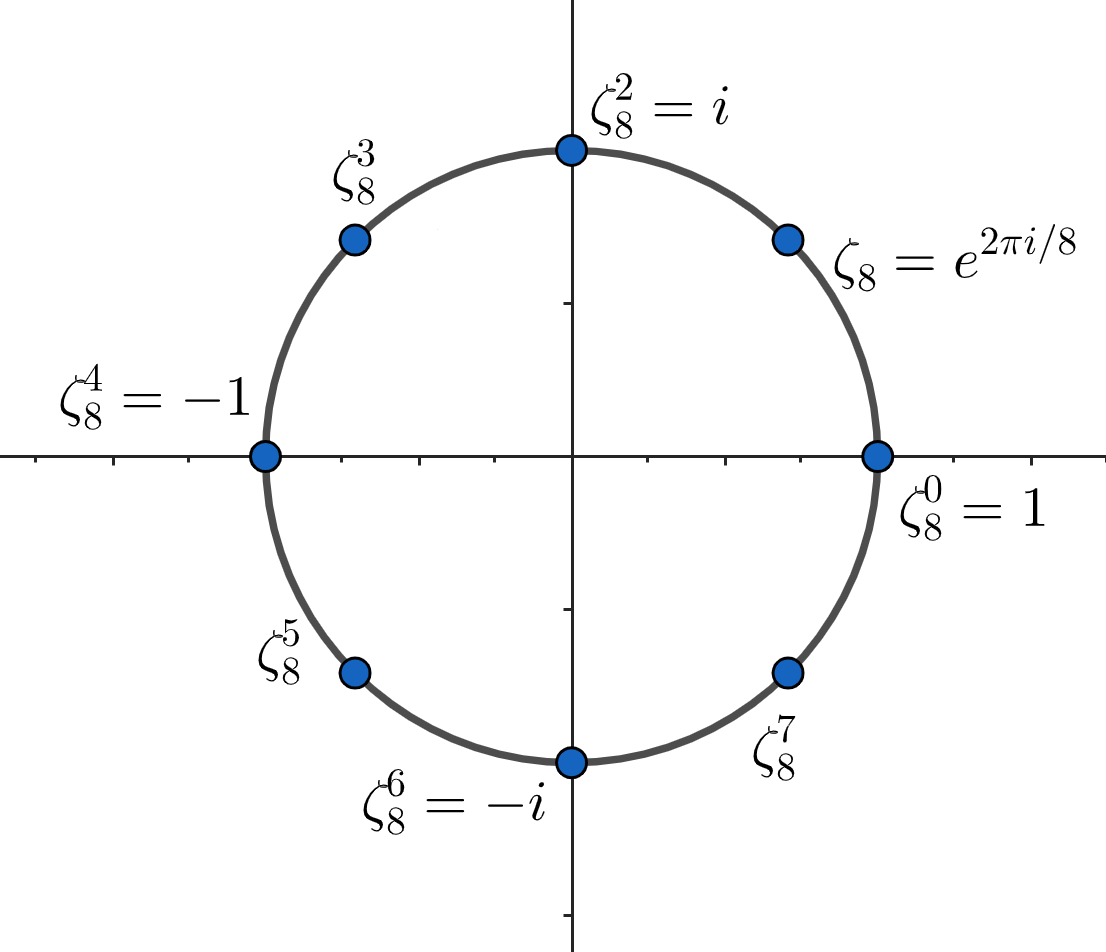
\includegraphics[scale=0.4]{files/figures/roots_of_unity.png}
    \caption{$8^{th}$ roots of unity}
    \label{fig:roots_of_unity}
\end{figure}

\begin{definition}[Primitive roots of unity]\cite{brilliant}
The $n^{th}$ primitive roots of unity are:
$$\{\zeta \in \mathbb C;\zeta^n=1\text{ and }\zeta^k\neq1,\forall ~ k<n \},$$
for positive integers $k$. They are the subset of $n^{th}$ roots of unity which are not $k^{th}$ roots of unity, for all $k<n$. They can be alternatively defined as:
$$\{\zeta_n^k;1\leq k \leq n,\gcd(k,n)=1\}$$
\end{definition}
From the Figure \ref{fig:roots_of_unity} example, the $8^{th}$ primitive roots of unity are $\zeta_8,\zeta_8^3,\zeta_8^5,\zeta_8^7$.
% Indeed, $\zeta_n^k=\exp(2k\pi i/n)$ will be equal to $1$ if, and only if the exponent is an integer multiple of $2\pi i$, which is not the case when $\gcd(k,n)=1$, since $k/n$
% tmp\cite{brilliant}

\begin{definition}[Cyclotomic polynomial] \label{def:cyclo}The \textit{$n$-th cyclotomical polynomial} is defined as:
\begin{align*}
    \Phi_n(x) = \prod_{\substack{1\leq k \leq n\\ \gcd(k,n)=1}}^{n}(x-\zeta_n^k)
\end{align*}
\end{definition}

Notice that its roots are the $n^{th}$ primitive roots of unity.

Using the definition, we can derive some cyclotomical polynomials, for example $\Phi_1(x)=x-1$ trivially, and $\Phi_2(x)=x+1$, since from the $2^{nd}$ roots of unity $-1$ and $+1$, only $-1$ are primitive ones.

The $3^{rd}$ primitive roots of are $\zeta_3^1$ and $\zeta_3^2=\overline{\zeta_3^1}$, then:
\begin{align}
    \Phi_3(x)&=(x-\zeta_3^1)(x-\zeta_3^2)\nonumber\\
    &=x^2-x(\zeta_3^1+\zeta_3^2)+\zeta_3^1\zeta_3^2\nonumber\\
    &=x^2-x(\zeta_3^1+\overline{\zeta_3^1})+e^{2\pi i(1+2)/3}\label{eq:zeta3}\nonumber\\
    &=x^2-x(2\cdot\cos(2\pi/3))+e^{2\pi i}\\
    &=x^2+x\left(2\cdot \frac12\right)+1\nonumber\\
    &=x^2+x+1\nonumber
\end{align}

The equality (1) holds due to the sum of complex conjugates being equal to two times the real part since we cancel out the imaginary terms.

\begin{theorem} For all positive integers $n$ we have:
$$\displaystyle x^n-1=\prod_{d|n}\Phi_d(x)$$
\end{theorem}

The above theorem provides a analytical formula to recursively generate the cyclotomic polynomials:
$$\displaystyle\Phi_n(x)=\dfrac{x^n-1}{\displaystyle\prod_{\substack{d|n\\d\neq n}}\Phi_d(x)}$$

We can use it to derive simpler, and non-recursive expressions for particular interesting cases:

\begin{corollary}[Prime Cyclotomical Polynomial]
If $p$ is a prime number, then:
$$\Phi_p(x)=x^{p-1}+x^{p-2}+\ldots+x+1$$
\end{corollary}

\begin{proof}
By the previous theorem, and the fact that the only $d<p$ satisfying $d|n$ is $d=1$:

$$\Phi_p(x)=\dfrac{x^p-1}{\displaystyle\prod_{\substack{d|p\\d\neq p}}\Phi_d(x)}=\dfrac{x^p-1}{\Phi_1(x)}=\dfrac{x^p-1}{x-1}$$

The polynomial division algorithm concludes that such a division actually results in what is claimed in the corollary.

An easy way to assert it, is by multiplying the divisor $x-1$ by $\displaystyle\sum_{i=0}^{p-1}x^i$ and checking if it is equal to $x^p-1$:
\begin{align*}
    (x-1)\left(\sum_{i=0}^{p-1}x^i\right)&=\sum_{i=0}^{p-1}x^{i+1}-\sum_{i=0}^{p-1}x^i\\
    &=\sum_{i=0}^{p-1}x^{i+1}-x^{i}\\
    &=x^{(p-1)+1}-x^{0}\\
    &=x^{p}-1
\end{align*}
\end{proof}
The following formula will be crucial to instantiate plaintext and cyphertext spaces in the encryption schemes.
\begin{corollary}[Power of Two Cyclotomic Polynomial]

\end{corollary}
\section{Lattices}

\section{LWE and RLWE}

\chapter{Homomorphic Encryption}

\section{Privacy Homomorphisms}

Assume we can represent the unencrypted data by an algebraic structure $\mathcal P= (S;f_1,\ldots,f_k)$, i.e., a set $S$ ported with the operations $f_1,\ldots,f_k$. We will further call this structure the plaintext space.

An alternative algebraic structure, the cyphertext space $\Cypher=(S',f'_1,\ldots,f'_k)$, is constructed to represent the encrypted data. To build a \textit{privacy homomorphism} \cite{Rivest1978},  one needs a decryption function $\phi:S'\to S$ and its inverse $\phi^{-1}:S\to S'$ satisfying the homomorphic property from $\Cypher$ do $\Plain$:
\begin{align}
    \label{privhom}
    f'_i(a,b,\ldots)&=c\Rightarrow\nonumber\\ f_i(\phi(a),\phi(b),\ldots)&=\phi(c),\text{ for } i=1,\ldots,k\\
    \text{with }a,b,&\ldots\in S'\nonumber
\end{align}
This means that for all available operations $f'_i$, its evaluation on encrypted elements must result in a value that, after decryption, corresponds to the same computation on the unencrypted domain.

An example of privacy homomorphism is the RSA cryptosystem \cite{rsa}, which uses $\Plain = (\Z_p;\times_p)$, the integers modulo $p$ with $p$ prime, and the multiplication modulo $p$. Setting $N=pq$, where $q$ is a large prime and choosing $e$ coprime with $(p-1)(q-1)$,  the cyphertext space as $(\Z_N;\times_N)$ and is connected with $\Plain$ through the encryption function:
\begin{align*}
    \phi^{-1}&:\Z_p\to\Z_N\\
    \phi^{-1}(x)&=x^e(\bmod N)
\end{align*}
Taking $x,y\in\Z_p$ and its encrypted versions $x'=\phi^{-1}(x),~y'=\phi^{-1}(y)$, we have:
\begin{align*}
    x'\times_N y'&= (x^e)(y^e)(\bmod N)\\
    &=(xy)^e(\bmod N),
\end{align*}
which is an encryption of $xy$. Then the multiplication satisfies property \ref{privhom}, showing that such a system is indeed a privacy homomorphism.

\subsection{Requirements and Limitations}
The following properties for $\Cypher,\phi$ and $\phi^{-1}$ are required by the authors:
\begin{alineas}
    \item for a given element $s\in S$, its encrypted version $\phi^{-1}(s)$ should not require much more storage space;
    \item $\phi$ and $\phi^{-1}$ should be easy to compute;
    \item the operations $f_i'$ should be efficiently computable in $\Cypher$;
    \item $\phi$ should not be vulnerable to the chosen plaintext attack;
    \item The operations of $\Cypher$ should not be sufficient to yield an efficient computation of $\phi$.
\end{alineas}

The last requirement forces a critical restriction on such morphisms: a comparison operator ``$\leq$'' can't be available in the cyphertext space, otherwise, no secure privacy homomorphism exists.

Take for example $\Plain = (\N;+,\leq)$ and $\Cypher = (W;+',\leq')$ for some $W$. A malicious party who has $\phi^{-1}(n)$, and wants to discover what $n\in\N$ generated such cyphertext can apply the following binary search strategy:
\begin{alineas}
\item compute $1'=\phi^{-1}(1)$;
\item compute $2'=1'+'1'$, then $4'=2'+'2'$;
\item continue until finding $k$, such that $\phi^{-1}(n)\leq'(2^k)'=\phi^{-1}(2^k)$
\item knowing that $n\in[2^{k-1},2^{k}]$, compute an encryption of the interval midpoint $\phi^{-1}(m)=\phi^{-1}(2^{k-1}-2^{k-2})$;
\item homomorphically compare $\phi^{-1}(n)\leq'\phi^{-1}(2^{k-1})+'\phi^{-1}(m)$;
\item repeat the last two steps properly redefining the interval until getting $n$ exactly.
\end{alineas}
This is an efficient $O(\log n)$ algorithm to compute the decryption function $\phi$, using the operations in $\Cypher$ and the ability to generate encryptions of arbitrary constants (such as $1$ and $m$ in the above example).

The article finishes with the authors pondering if such an approach with all required security restrictions could be worthwhile in practice and what algebraic structures $\Plain$ would provide usefuls privacy homomorphisms.
% \section{First Generation Fully Homomorphic schemes}
% \begin{alineas}
% \item somewhat/fully homomorphic
% \item bootstrapping
% \item integer scheme
% \item caveats and implementation paper
% \end{alineas}

\section{Fully Homomorphic Encryption}
\section{Gentry's work}


\subsection{BFV and BGV schemes (integers)}

\begin{alineas}
\item describe BFV primitives (codec/ring)
\item encrypt/decrypt
\item relinelization
\item BGV differences
\end{alineas}

\subsection{CKKS scheme (complex numbers)}

- brief description about fixed point arithmetic?
- the complex map 
- 
\subsection{Approximate Bootstrapping}

\chapter{Private Logistic Regression}
\section{Statistical Review}
\section{Homomorphic Training}
\section{Data Applications}


\label{ch:algebra}



\chapter{Conclusions}
\label{ch:conclusions}




% -----------------------------------
% ELEMENTOS PÓS-TEXTUAIS
% -----------------------------------
\postextual
% ----------------------------------

%\bibliography{biblio}
\printbibliography

%\glossary

% ----------------------------------------------------------
% Apêndices
% ----------------------------------------------------------

\begin{apendicesenv}

\partapendices

\chapter{An ideal lattice scheme}
\label{appendixA}
\section{Initial definitions}

\begin{definition}[Relatively Prime Ideals]
Two ideals $I$ and $J$ of a ring $R$ are considered relatively primes if $I+J=R$, where $I+J=\{i+j|i\in I,j\in J\}$.
\end{definition}

\begin{definition}[Half-open parallelepiped]
For a given lattice basis $\mathbf B$, we define the half-open parallelepiped $\mathcal P (\mathbf B)$ as:
$$\mathcal P (\mathbf B)=\Big\{\sum_{i=1}^{n}x_ib_i\left|\right. x_i\in [-1/2,1/2)\Big\}$$
\end{definition}

\begin{proposition}
For a given $\mathbf t \in\mathbb{R}^n$, there exists an unique $\mathbf t'\in\mathcal P(\mathbf B)$, such that, $\mathbf t-\mathbf t' \in\mathcal L(\mathbf B)$ we define the operation of ``reduction modulo the basis'' as the map from $\mathbf t$ to $\mathbf t'$.
\begin{align*}
    \mod \mathbf B:\mathbb{R}^n&\to\mathcal P(\mathbf B)\\
    \mod \mathbf B:\mathbf t &\mapsto \mathbf t \bmod \mathbf B := \mathbf t'
\end{align*}

This operation can be computed as:
$$\mathbf t\bmod \mathbf B=\mathbf t-\mathbf B\cdot\lfloor{\mathbf B}^{-1}\cdot\mathbf t\rceil,$$

where $\lfloor.\rceil$ round the entry to the closest integer. \cite{stan16}
\end{proposition}

\section{An abstract construction}
Gentry \cite{gentry2009fully} proposes an abstract scheme before making reference to ideal lattices. We need the following components:

\begin{itemize}
    \item $R$ - a fixed ring;
    \item $\mathbf B_I$ - a fixed basis of an ideal $I\in R$;
    \item $\operatorname{IdealGen}(R,\mathbf B_I)$ - an algorithm that outputs $\mathbf B_{J}^{pk},\mathbf B_{J}^{sk}$, public and secret basis of an ideal $J$, such that $I$ and $J$ are relatively prime ideals.
    \item $\operatorname{Samp}(\mathbf B_I,x)$ - a function that samples from the coset $x+I$.
\end{itemize}

The scheme can be proved secure if we use the function $\operatorname{Samp}(\mathbf B_I,x)=x+r\times s$, where $r$ is chosen randomly from $R$, $I$ is a principal ideal and $s$ its generator.

Moreover, we assume that for every $\mathbf t \in R$, and a given basis $\mathbf B_M$ of an ideal $M\subset R$, there exists an unique representative $\mathbf t \bmod {\mathbf B_M}$, that can be efficiently computed.

Then we can construct a (somewhat) homomorphic encryption scheme, using the functions $\operatorname{KeyGen}$, $\enc$, $\dec$, and $\eval$:
\begin{itemize}
    \item $\operatorname{KeyGen}(R,\mathbf B_I)$ - sets public and secret basis $(\mathbf B_{J}^{pk},\mathbf B_{J}^{sk})\leftarrow \operatorname{IdealGen}(R,\mathbf{B_I})$. Then the public key is $\operatorname{pk}=(R,\mathbf B_I,\mathbf B_J^{pk},\operatorname{Samp})$ and secret key includes the secrete basis $\operatorname{sk}=(R,\mathbf B_I,\mathbf B_j^{pk},\operatorname{Samp},\mathbf B_J^{sk})$
    \item $\enc(\operatorname{pk},\pi)=\operatorname{Samp}(\mathbf B_I,\pi)\bmod \mathbf B_J^{pk}$
    
    \item $\dec(\operatorname{sk},\psi) = (\psi \bmod \mathbf B_J^{sk})\bmod \mathbf{B_I}$
    
    \item $\eval(\operatorname{pk},F,\Psi)$ - takes a circuit $F$ of additions and multiplications $\bmod$-$ \mathbf B_I$ and invoked Add and Mult below, in the proper order.
    \begin{align*}
        \operatorname{Add}(pk,\psi_1,\psi_2)=\psi_1+\psi_2\bmod\mathbf B_J^{pk}\\
        \operatorname{Mult}(pk,\psi_1,\psi_2)=\psi_1\times\psi_2\bmod\mathbf B_J^{pk}
    \end{align*}
\end{itemize}

More generally, given a circuit $F$ of addition and multiplications  $\bmod$-$ \mathbf B_I$, the $\eval$ function is:
$$\eval(\operatorname{pk},F,\Psi)=g(F)(\Psi)\bmod\mathbf B_J^{pk},$$

where $g(F)$ is the generalized circuit that replaces $\operatorname{Add}_{\mathbf{B_I}}$ and $\operatorname{Mult}_{\mathbf{B_I}}$ by ``$+$'' and ``$\times$'' operations of the ring $R$.

Its not trivial that correctness property (\ref{eq:correctness}). In fact, it holds only for a specific group of circuits.

Let's define $X_{Enc}$ as the image of $\operatorname{Samp}$ and $X_{Dec}=R\bmod\mathbf{B_J^{sk}}$, i.e, the set of indistinguishable representatives of cosets of $J$.

We call $\mathcal{F_E}$ a set of \textbf{permitted circuits} if its a subset of
$$\{F:\forall (x_1,\ldots,x_n)\in X_{Enc}, g(F)(x_1,\ldots,x_n)\in X_{Dec}\},$$

i.e., the set of $\bmod$-$\mathbf B_I$ circuits such that its generalization is in $X_{Dec}$ when the input is in $X_{Enc}$. For the permitted circuits, one can prove that homomorphic decryption works correctly.

\section{A concrete construction using ideal lattices}

Let $f\in\mathbb{Z}[x]$ be a monic polynomial of degree $n$ and define the ring:
$$R=\mathbb{Z}[x]/(f)$$

whose elements can be uniquely represent by:

$$\Big\{\overline{\displaystyle\sum_{i=1}^{n}\alpha_ix^{i-1}}|\alpha_i\in\mathbb Z\Big\},$$
where $\overline{P(x)}=P(x)\bmod f(x)$, i.e, the remainder in the polynomial division of $P$ by $f$. Since $\deg(f)=n$, the polynomials in the above set have degrees up to $n-1$. So, there is a bijective map $\varphi:R\to\mathbb{Z}^n$, that takes $r=\sum_{i=1}^{n}\alpha_ix^{i-1}\in R$ and makes $\varphi(r)=(\alpha_1,\ldots,\alpha_n)^T$

Let $v\in R$ be a generator of an ideal $J$. We can construct an ideal lattice using the so-called \textit{rotation basis} $\mathbf{B_J}$ with columns: 
\begin{align*}
    b_i&=\varphi(b_i^*),\\ 
    \text{where } b_i^*&=v\times x^{i-1}\bmod f(x)
\end{align*}
One can easily prove that there is a bijection between $J$ and $\mathcal{L}(\mathbf{B_J})$.
\begin{lemma}
\label{reduction}
Let $r\in\mathbb{Z}^n,~j\in\mathcal{L}(\mathbf{B_J})$ where $J$ is an ideal of $R=\mathbb{Z}[x]/(f)$. Then:
$$(r+j)\bmod \mathbf{B_J}=r\bmod \mathbf{B_J}$$
\end{lemma}

Gentry's original scheme, starts with $R$, an ideal $I$, and $\mathbf{B_I}$ a basis of $\mathcal{L}(\mathbf{B_I})$ (not necessarily the rotation one). Then the algorithm $\operatorname{IdealGen}$ described in previous section, chooses another ideal $J$ such that $I$ and $J$ are relatively primes, and outputs $\mathbf{B_J^{pk}},\mathbf{B_J^{sk}}$ basis of $\mathcal{L}_J$. A possible choice for the secret basis in the rotation one, and for the public basis, one can use the hermite normal form of $\mathbf{B_J^{sk}}$. 

The algorithms $\enc,\dec$ and $\eval$ works as described before. 

Using ideal lattices, we can redefine $X_{Enc}$ and $X_{Dec}$ here in order to obtain a geometric interpretation. At first, notice that $X_{Dec}=R\bmod\mathbf{B_J^{sk}}=\mathcal{P}(B_J^{sk})$.

Let $\mathcal{B}(r)$ be the origin centered ball in $\mathbb{R}^n$ with radius $r$. Then, defines:
\begin{itemize}
    \item $r_{Enc}$ - a value s.t.  $\mathcal{B}(r_{Enc})$ is the smallest ball satisfying  $X_{Enc}\subseteq\mathcal{B}(r_{Enc})$
    \item $r_{Dec}$ - a value s.t. $\mathcal{B}(r_{Dec})$ is the greatest ball satisfying $\mathcal{B}(r_{Dec})\subseteq X_{Dec}=\mathcal{P}(\mathbf{B_J^{sk}})$
\end{itemize}
Now the set of permitted circuits become:
$$\mathcal{F_E}=\{F:\forall (x_1,\ldots,x_n)\in \mathcal{B}(r_{Enc}), g(F)(x_1,\ldots,x_n)\in \mathcal{B}(r_{Dec})\}$$

Fixed $r_{Enc},r_{Dec}$ we want to know what is $\mathcal{C_E}$. We can bound $||g(F)(x_1,\ldots,x_n)||$ by bounding $||u+v||$ and $||u\times v||$. We know that $||u+v||\leq ||u||+||v||$, by the triangle inequality. One can explicit a factor $\gamma_{Mult}(R)$, depending only on the ring, s.t. $||u\times v||\leq\gamma_{Mult}(R)(||u||\times||v||)$.
Then, Gentry shows that the scheme correctly evaluates any circuit $F$ with depth at most
$$\log\log r_{Dec}-\log\log(\gamma_{Mult}(R)\cdot r_{Enc})$$

Then the author dedicates a lot of chapters show tweaks to  simplifying the decryption circuit complexity, such that the scheme can evaluate it, and a bootstrappable scheme is achieved.

It's desirable to maximize $r_{Dec}$, and minimize $r_{Enc}$ and $\gamma_{Mult}(R)$. Gentry's work show that:
\begin{align*}
    r_{Dec}&=\dfrac{1}{2||\mathbf{B_J^{sk*}}||},\text{ where }\\
    \mathbf{B_J^{sk*}}&=((\mathbf{B_J^{sk}})^{-1})^T
\end{align*}
Also, by choosing $R=\mathbb{Z}[x]/(f)$ with $f(x)=x^n-1$, then it can be proved that:
$$\gamma_{Mult}(R)\leq\sqrt{n}$$

Now we'll prove that our SHE scheme correctly decrypts a \textit{valid cyphertext} (a cyphertext that can be outputed by $\enc$ or $\eval$).


\begin{theorem}[\textbf{Identity correctness}] 
\label{correctness_thm} Consider $\pi \in \Pi$, where $\Pi=\{\pi|\pi\in\mathcal{P}(\mathbf{ B_I})\}$ is the plaintext space. If $\operatorname{Samp}(\pi)\in\mathcal{B}(r_{Dec})$, then 
$$\dec(sk,\enc(pk,\pi))=\pi$$ 
\end{theorem}
\begin{proof}
The cyphertext is 
\begin{align*}
    \psi &= \operatorname{Samp}(\mathbf{B_I},\pi)\bmod \mathbf{B_J^{pk}}\\
    &= (\pi+i)\bmod \mathbf{B_J^{pk}},
\end{align*}
for some $i\in\mathcal{L}_I$. We can write $\psi=\pi+i+j$, for some $j\in\mathcal{L}_J$ because:
\begin{align*}
    \psi&=(\pi+i)\bmod \mathbf{B_J^{pk}}\\
    &=(\pi + i)-\mathbf{B_J^{pk}}\times c,
\end{align*}
where $c=\lfloor(\mathbf{B_J^{pk}})^{-1}(\pi+i)\rceil$. Since $c\in\mathbb{Z}^k$, if $j=\mathbf{B_J^{pk}}\times (-c)$, then $j\in\mathcal{L}_J$, by definition of lattice.

Then, by using Lemma \ref{reduction} and the fact that $(\pi+i)\in\mathcal{B}(r_{Dec})\subseteq\mathcal{P}(\mathbf{B}_J^{sk})$:

\begin{align*}
    &~~~\dec(sk,\enc(pk,\pi))\\&=\dec(sk,\psi)\\
    &=((\pi+i+j)\bmod\mathbf{B}_J^{sk})\bmod\mathbf{B}_I\\
    &=((\pi+i)\bmod\mathbf{B}_J^{sk})\bmod\mathbf{B}_I\\
    &=(\pi+i)\bmod\mathbf{B}_I\\
    &=\pi
\end{align*}
\end{proof}





\end{apendicesenv}

% ----------------------------------------------------------
% Anexos
% ----------------------------------------------------------

% \begin{anexosenv}

% \partanexos

% \end{anexosenv}

%---------------------------------------------------------------------
% ÍNDICE REMISSIVO
%---------------------------------------------------------------------
\phantompart
\printindex

\end{document}